\documentclass[]{article}
\usepackage{lmodern}
\usepackage{amssymb,amsmath}
\usepackage{ifxetex,ifluatex}
\usepackage{fixltx2e} % provides \textsubscript
\ifnum 0\ifxetex 1\fi\ifluatex 1\fi=0 % if pdftex
  \usepackage[T1]{fontenc}
  \usepackage[utf8]{inputenc}
\else % if luatex or xelatex
  \ifxetex
    \usepackage{mathspec}
  \else
    \usepackage{fontspec}
  \fi
  \defaultfontfeatures{Ligatures=TeX,Scale=MatchLowercase}
\fi
% use upquote if available, for straight quotes in verbatim environments
\IfFileExists{upquote.sty}{\usepackage{upquote}}{}
% use microtype if available
\IfFileExists{microtype.sty}{%
\usepackage{microtype}
\UseMicrotypeSet[protrusion]{basicmath} % disable protrusion for tt fonts
}{}
\usepackage[margin=1in]{geometry}
\usepackage{hyperref}
\hypersetup{unicode=true,
            pdftitle={Datasets},
            pdfborder={0 0 0},
            breaklinks=true}
\urlstyle{same}  % don't use monospace font for urls
\usepackage{color}
\usepackage{fancyvrb}
\newcommand{\VerbBar}{|}
\newcommand{\VERB}{\Verb[commandchars=\\\{\}]}
\DefineVerbatimEnvironment{Highlighting}{Verbatim}{commandchars=\\\{\}}
% Add ',fontsize=\small' for more characters per line
\usepackage{framed}
\definecolor{shadecolor}{RGB}{248,248,248}
\newenvironment{Shaded}{\begin{snugshade}}{\end{snugshade}}
\newcommand{\AlertTok}[1]{\textcolor[rgb]{0.94,0.16,0.16}{#1}}
\newcommand{\AnnotationTok}[1]{\textcolor[rgb]{0.56,0.35,0.01}{\textbf{\textit{#1}}}}
\newcommand{\AttributeTok}[1]{\textcolor[rgb]{0.77,0.63,0.00}{#1}}
\newcommand{\BaseNTok}[1]{\textcolor[rgb]{0.00,0.00,0.81}{#1}}
\newcommand{\BuiltInTok}[1]{#1}
\newcommand{\CharTok}[1]{\textcolor[rgb]{0.31,0.60,0.02}{#1}}
\newcommand{\CommentTok}[1]{\textcolor[rgb]{0.56,0.35,0.01}{\textit{#1}}}
\newcommand{\CommentVarTok}[1]{\textcolor[rgb]{0.56,0.35,0.01}{\textbf{\textit{#1}}}}
\newcommand{\ConstantTok}[1]{\textcolor[rgb]{0.00,0.00,0.00}{#1}}
\newcommand{\ControlFlowTok}[1]{\textcolor[rgb]{0.13,0.29,0.53}{\textbf{#1}}}
\newcommand{\DataTypeTok}[1]{\textcolor[rgb]{0.13,0.29,0.53}{#1}}
\newcommand{\DecValTok}[1]{\textcolor[rgb]{0.00,0.00,0.81}{#1}}
\newcommand{\DocumentationTok}[1]{\textcolor[rgb]{0.56,0.35,0.01}{\textbf{\textit{#1}}}}
\newcommand{\ErrorTok}[1]{\textcolor[rgb]{0.64,0.00,0.00}{\textbf{#1}}}
\newcommand{\ExtensionTok}[1]{#1}
\newcommand{\FloatTok}[1]{\textcolor[rgb]{0.00,0.00,0.81}{#1}}
\newcommand{\FunctionTok}[1]{\textcolor[rgb]{0.00,0.00,0.00}{#1}}
\newcommand{\ImportTok}[1]{#1}
\newcommand{\InformationTok}[1]{\textcolor[rgb]{0.56,0.35,0.01}{\textbf{\textit{#1}}}}
\newcommand{\KeywordTok}[1]{\textcolor[rgb]{0.13,0.29,0.53}{\textbf{#1}}}
\newcommand{\NormalTok}[1]{#1}
\newcommand{\OperatorTok}[1]{\textcolor[rgb]{0.81,0.36,0.00}{\textbf{#1}}}
\newcommand{\OtherTok}[1]{\textcolor[rgb]{0.56,0.35,0.01}{#1}}
\newcommand{\PreprocessorTok}[1]{\textcolor[rgb]{0.56,0.35,0.01}{\textit{#1}}}
\newcommand{\RegionMarkerTok}[1]{#1}
\newcommand{\SpecialCharTok}[1]{\textcolor[rgb]{0.00,0.00,0.00}{#1}}
\newcommand{\SpecialStringTok}[1]{\textcolor[rgb]{0.31,0.60,0.02}{#1}}
\newcommand{\StringTok}[1]{\textcolor[rgb]{0.31,0.60,0.02}{#1}}
\newcommand{\VariableTok}[1]{\textcolor[rgb]{0.00,0.00,0.00}{#1}}
\newcommand{\VerbatimStringTok}[1]{\textcolor[rgb]{0.31,0.60,0.02}{#1}}
\newcommand{\WarningTok}[1]{\textcolor[rgb]{0.56,0.35,0.01}{\textbf{\textit{#1}}}}
\usepackage{graphicx,grffile}
\makeatletter
\def\maxwidth{\ifdim\Gin@nat@width>\linewidth\linewidth\else\Gin@nat@width\fi}
\def\maxheight{\ifdim\Gin@nat@height>\textheight\textheight\else\Gin@nat@height\fi}
\makeatother
% Scale images if necessary, so that they will not overflow the page
% margins by default, and it is still possible to overwrite the defaults
% using explicit options in \includegraphics[width, height, ...]{}
\setkeys{Gin}{width=\maxwidth,height=\maxheight,keepaspectratio}
\IfFileExists{parskip.sty}{%
\usepackage{parskip}
}{% else
\setlength{\parindent}{0pt}
\setlength{\parskip}{6pt plus 2pt minus 1pt}
}
\setlength{\emergencystretch}{3em}  % prevent overfull lines
\providecommand{\tightlist}{%
  \setlength{\itemsep}{0pt}\setlength{\parskip}{0pt}}
\setcounter{secnumdepth}{0}
% Redefines (sub)paragraphs to behave more like sections
\ifx\paragraph\undefined\else
\let\oldparagraph\paragraph
\renewcommand{\paragraph}[1]{\oldparagraph{#1}\mbox{}}
\fi
\ifx\subparagraph\undefined\else
\let\oldsubparagraph\subparagraph
\renewcommand{\subparagraph}[1]{\oldsubparagraph{#1}\mbox{}}
\fi

%%% Use protect on footnotes to avoid problems with footnotes in titles
\let\rmarkdownfootnote\footnote%
\def\footnote{\protect\rmarkdownfootnote}

%%% Change title format to be more compact
\usepackage{titling}

% Create subtitle command for use in maketitle
\providecommand{\subtitle}[1]{
  \posttitle{
    \begin{center}\large#1\end{center}
    }
}

\setlength{\droptitle}{-2em}

  \title{Datasets}
    \pretitle{\vspace{\droptitle}\centering\huge}
  \posttitle{\par}
    \author{}
    \preauthor{}\postauthor{}
    \date{}
    \predate{}\postdate{}
  

\begin{document}
\maketitle

\hypertarget{binary}{%
\section{Binary}\label{binary}}

\begin{itemize}
\tightlist
\item
  \textbf{Binary}

  \begin{itemize}
  \tightlist
  \item
    Categorical attributes

    \begin{itemize}
    \tightlist
    \item
      Less than 10 attributes

      \begin{itemize}
      \tightlist
      \item
        \protect\hyperlink{Balance-Scale}{Balance Scale}
      \item
        \protect\hyperlink{Breast-Cancer}{Breast Cancer}
      \item
        \protect\hyperlink{Cars}{Cars}
      \item
        \protect\hyperlink{Tic-Tac-Toe}{Tic-Tac-Toe}
      \end{itemize}
    \item
      10 or more attributes
    \end{itemize}
  \item
    Mixed: categorical and numerical attributes

    \begin{itemize}
    \tightlist
    \item
      Less than 10 attributes
    \item
      10 or more attributes

      \begin{itemize}
      \tightlist
      \item
        \protect\hyperlink{Travel-insurance}{Travel Insurance}
      \end{itemize}
    \end{itemize}
  \item
    Numeric attributes

    \begin{itemize}
    \tightlist
    \item
      Less than 10 attributes

      \begin{itemize}
      \tightlist
      \item
        \protect\hyperlink{Weight-height-gender}{Weight, height, gender}
      \end{itemize}
    \item
      10 or more attributes
    \end{itemize}
  \end{itemize}
\item
  \textbf{Multiclass}

  \begin{itemize}
  \tightlist
  \item
    Categorical attributes

    \begin{itemize}
    \tightlist
    \item
      Less than 10 attributes

      \begin{itemize}
      \tightlist
      \item
        \protect\hyperlink{Post-operative}{Post-operative}
      \end{itemize}
    \item
      10 or more attributes
    \end{itemize}
  \item
    Mixed: categorical and numerical attributes

    \begin{itemize}
    \tightlist
    \item
      Less than 10 attributes
    \item
      10 or more attributes
    \end{itemize}
  \item
    Numeric attributes

    \begin{itemize}
    \tightlist
    \item
      Less than 10 attributes
    \item
      10 or more attributes
    \end{itemize}
  \end{itemize}
\end{itemize}

\hypertarget{binary-1}{%
\section{Binary}\label{binary-1}}

\hypertarget{categorical-attributes}{%
\subsection{Categorical attributes}\label{categorical-attributes}}

\hypertarget{Balance-Scale}{%
\paragraph{Balance Scale}\label{Balance-Scale}}

This data set was generated to model psychological experimental results.
Each example is classified as having the balance scale tip to the right,
tip to the left, or be balanced. The attributes are the left weight, the
left distance, the right weight, and the right distance. The correct way
to find the class is the greater of \((left\_distance * left\_weight)\)
and \((right\_distance * right\_weight)\). If they are equal, it is
balanced.

\begin{itemize}
\tightlist
\item
  \textbf{Source}:
  \href{http://archive.ics.uci.edu/ml/datasets/Balance+Scale}{UCI
  Machile Learning Repository}
\item
  \textbf{Number of rows}: 625
\item
  \textbf{Number of attributes}: 4
\end{itemize}

\textbf{Description of the attributes:}

\includegraphics[width=1\linewidth]{Datasets_files/figure-latex/unnamed-chunk-2-1}

\hypertarget{Breast-Cancer}{%
\paragraph{Breast Cancer}\label{Breast-Cancer}}

This is one of three domains provided by the Oncology Institute that has
repeatedly appeared in the machine learning literature.(See also
lymphography and primary-tumor.)

This data set includes 201 instances of one class and 85 instances of
another class. The instances are described by 9 attributes, some of
which are linear and some are nominal.

\begin{itemize}
\tightlist
\item
  \textbf{Source}:
  \href{http://archive.ics.uci.edu/ml/datasets/Breast+Cancer}{UCI
  Machile Learning Repository}
\item
  \textbf{Number of rows}: 277
\item
  \textbf{Number of attributes}: 9
\end{itemize}

\textbf{Description of the attributes:}

\includegraphics[width=1\linewidth]{Datasets_files/figure-latex/unnamed-chunk-3-1}

\hypertarget{Cars}{%
\paragraph{Cars}\label{Cars}}

Car Evaluation Database was derived from a simple hierarchical decision
model originally developed for the demonstration of DEX, M. Bohanec, V.
Rajkovic: Expert system for decision making. Sistemica 1(1),
pp.~145-157, 1990.). The model evaluates cars according to the following
concept structure:

CAR car acceptability . PRICE overall price . . buying buying price . .
maint price of the maintenance . TECH technical characteristics . .
COMFORT comfort . . . doors number of doors . . . persons capacity in
terms of persons to carry . . . lug\_boot the size of luggage boot . .
safety estimated safety of the car

Input attributes are printed in lowercase. Besides the target concept
(CAR), the model includes three intermediate concepts: PRICE, TECH,
COMFORT. Every concept is in the original model related to its lower
level descendants by a set of examples (for these examples sets see
{[}Web Link{]}).

The Car Evaluation Database contains examples with the structural
information removed, i.e., directly relates CAR to the six input
attributes: buying, maint, doors, persons, lug\_boot, safety. Because of
known underlying concept structure, this database may be particularly
useful for testing constructive induction and structure discovery
methods.

\begin{itemize}
\tightlist
\item
  \textbf{Source}:
  \href{http://archive.ics.uci.edu/ml/datasets/Car+Evaluation}{UCI
  Machile Learning Repository}
\item
  \textbf{Number of rows}: 1728
\item
  \textbf{Number of attributes}: 6
\end{itemize}

\textbf{Description of the attributes:}

\includegraphics[width=1\linewidth]{Datasets_files/figure-latex/unnamed-chunk-4-1}

\hypertarget{Tic-Tac-Toe}{%
\paragraph{Tic-Tac-Toe}\label{Tic-Tac-Toe}}

This database encodes the complete set of possible board configurations
at the end of tic-tac-toe games, where ``x'' is assumed to have played
first. The target concept is ``win for x'' (i.e., true when ``x'' has
one of 8 possible ways to create a ``three-in-a-row'').

\begin{itemize}
\tightlist
\item
  \textbf{Source}:
  \href{http://archive.ics.uci.edu/ml/datasets/Tic-Tac-Toe+Endgame}{UCI
  Machile Learning Repository}
\item
  \textbf{Number of rows}: 958
\item
  \textbf{Number of attributes}: 9
\end{itemize}

\textbf{Description of the attributes:}

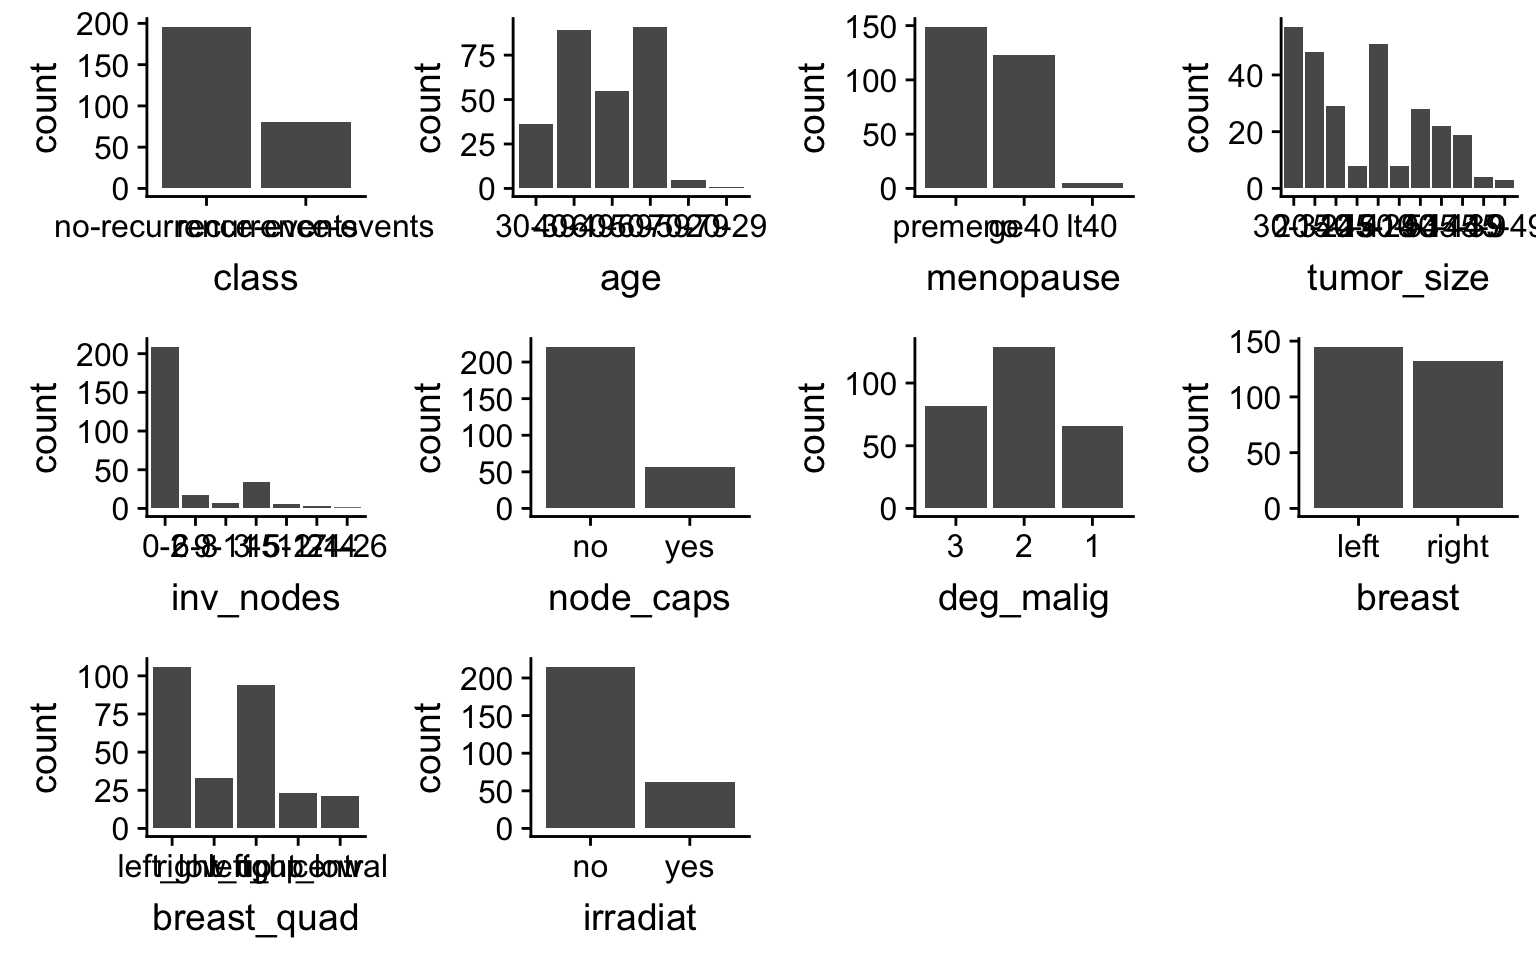
\includegraphics[width=1\linewidth]{Datasets_files/figure-latex/unnamed-chunk-5-1}

\hypertarget{less-than-10-attributes}{%
\subsubsection{Less than 10 attributes}\label{less-than-10-attributes}}

\hypertarget{or-more-attributes}{%
\subsubsection{10 or more attributes}\label{or-more-attributes}}

\hypertarget{mixed-categorical-and-numerical-attributes}{%
\subsection{Mixed: categorical and numerical
attributes}\label{mixed-categorical-and-numerical-attributes}}

\hypertarget{less-than-10-attributes-1}{%
\subsubsection{Less than 10
attributes}\label{less-than-10-attributes-1}}

\hypertarget{or-more-attributes-1}{%
\subsubsection{10 or more attributes}\label{or-more-attributes-1}}

\hypertarget{Travel-insurance}{%
\paragraph{Travel insurance}\label{Travel-insurance}}

\url{https://www.kaggle.com/mhdzahier/travel-insurance\#travel\%20insurance.csv}

\begin{Shaded}
\begin{Highlighting}[]
\KeywordTok{plot_dist_cols}\NormalTok{(travel_insurance)}
\end{Highlighting}
\end{Shaded}

\begin{verbatim}
## `stat_bin()` using `bins = 30`. Pick better value with `binwidth`.
## `stat_bin()` using `bins = 30`. Pick better value with `binwidth`.
## `stat_bin()` using `bins = 30`. Pick better value with `binwidth`.
## `stat_bin()` using `bins = 30`. Pick better value with `binwidth`.
\end{verbatim}

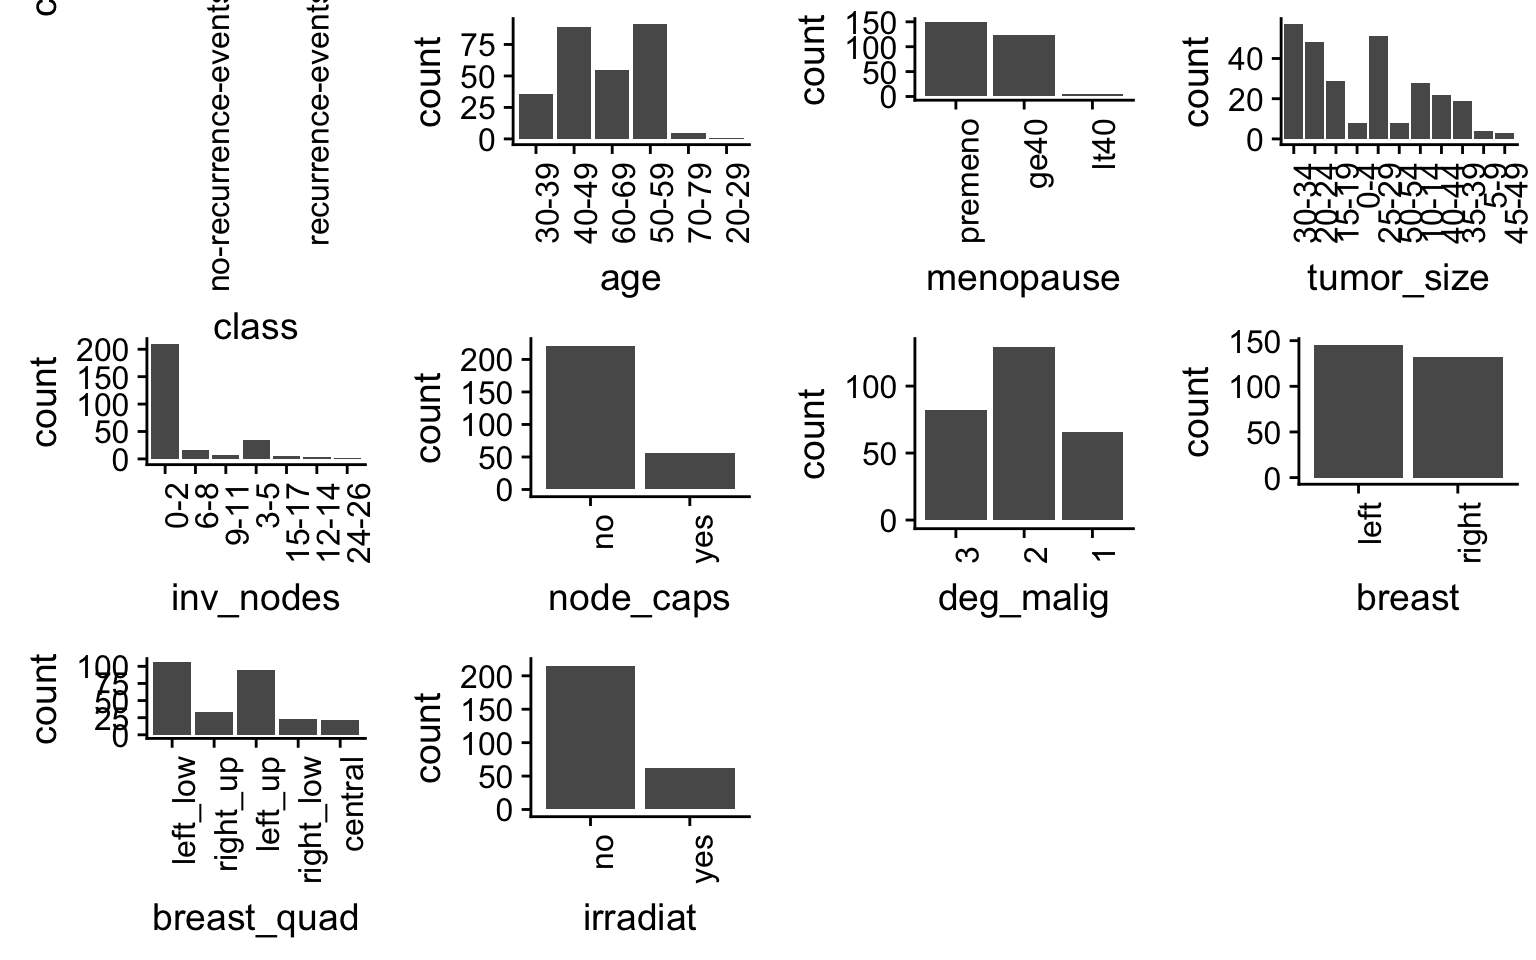
\includegraphics[width=1\linewidth]{Datasets_files/figure-latex/unnamed-chunk-6-1}

\hypertarget{numeric-attributes}{%
\subsection{Numeric attributes}\label{numeric-attributes}}

\hypertarget{less-than-10-attributes-2}{%
\subsubsection{Less than 10
attributes}\label{less-than-10-attributes-2}}

\hypertarget{or-more-attributes-2}{%
\subsubsection{10 or more attributes}\label{or-more-attributes-2}}

\begin{center}\rule{0.5\linewidth}{\linethickness}\end{center}

\hypertarget{multiclass}{%
\section{Multiclass}\label{multiclass}}

\hypertarget{categorical-attributes-1}{%
\subsection{Categorical attributes}\label{categorical-attributes-1}}

\hypertarget{less-than-10-attributes-3}{%
\subsubsection{Less than 10
attributes}\label{less-than-10-attributes-3}}

\hypertarget{Post-operative}{%
\paragraph{Post operative data}\label{Post-operative}}

\begin{Shaded}
\begin{Highlighting}[]
\KeywordTok{plot_dist_cols}\NormalTok{(post_operative)}
\end{Highlighting}
\end{Shaded}

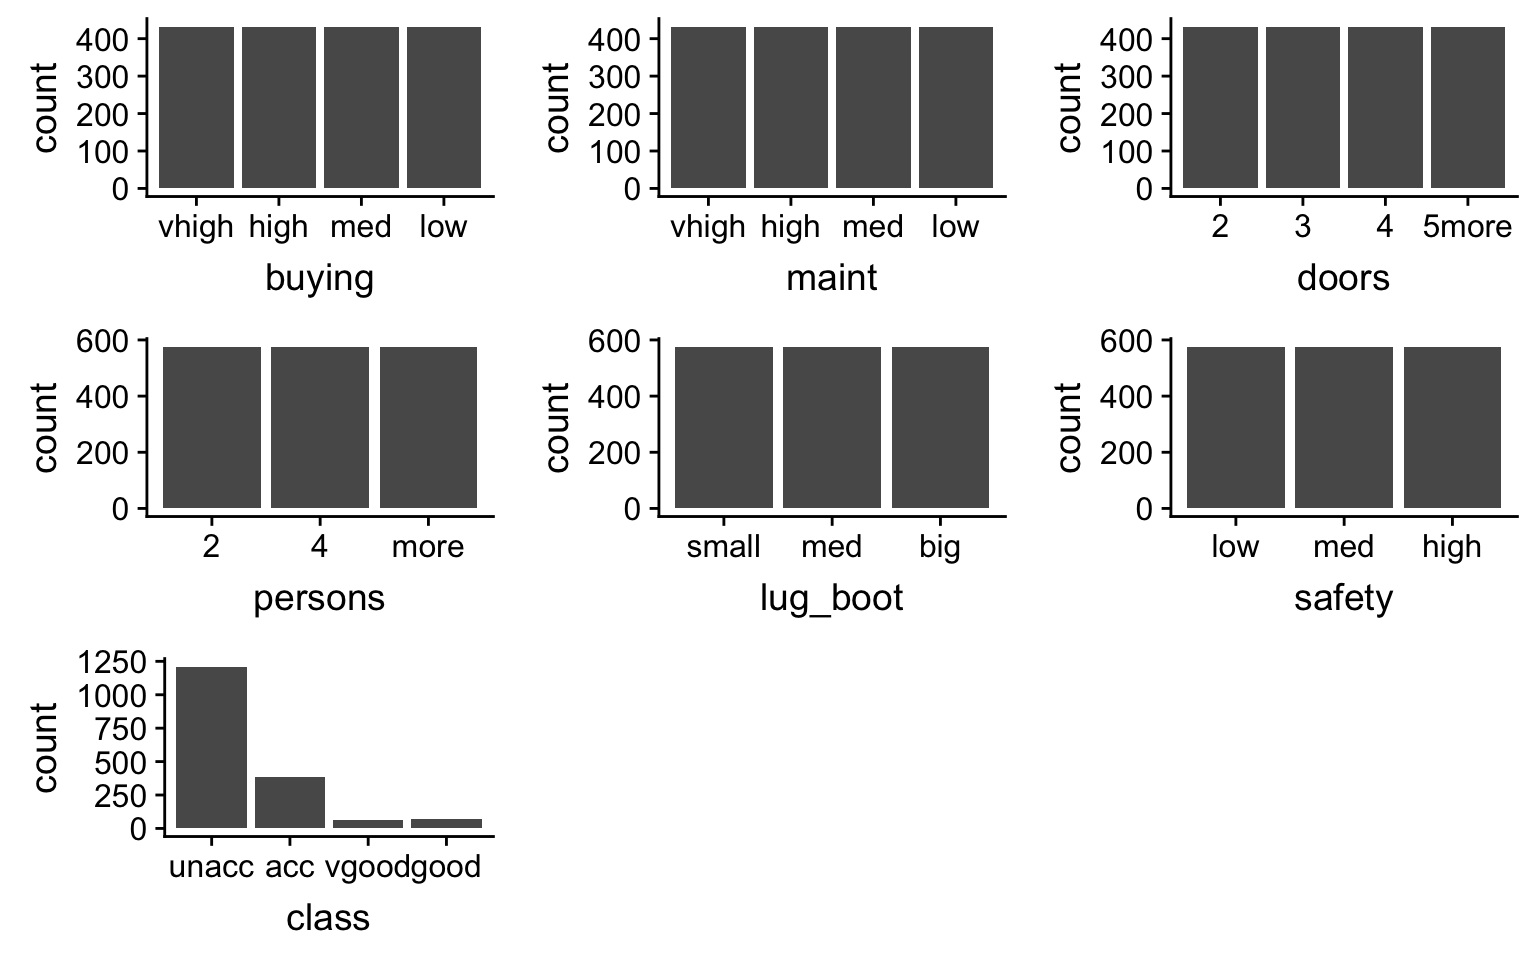
\includegraphics[width=1\linewidth]{Datasets_files/figure-latex/unnamed-chunk-7-1}

\hypertarget{or-more-attributes-3}{%
\subsubsection{10 or more attributes}\label{or-more-attributes-3}}

\hypertarget{Poker-hand}{%
\paragraph{Poker hand}\label{Poker-hand}}

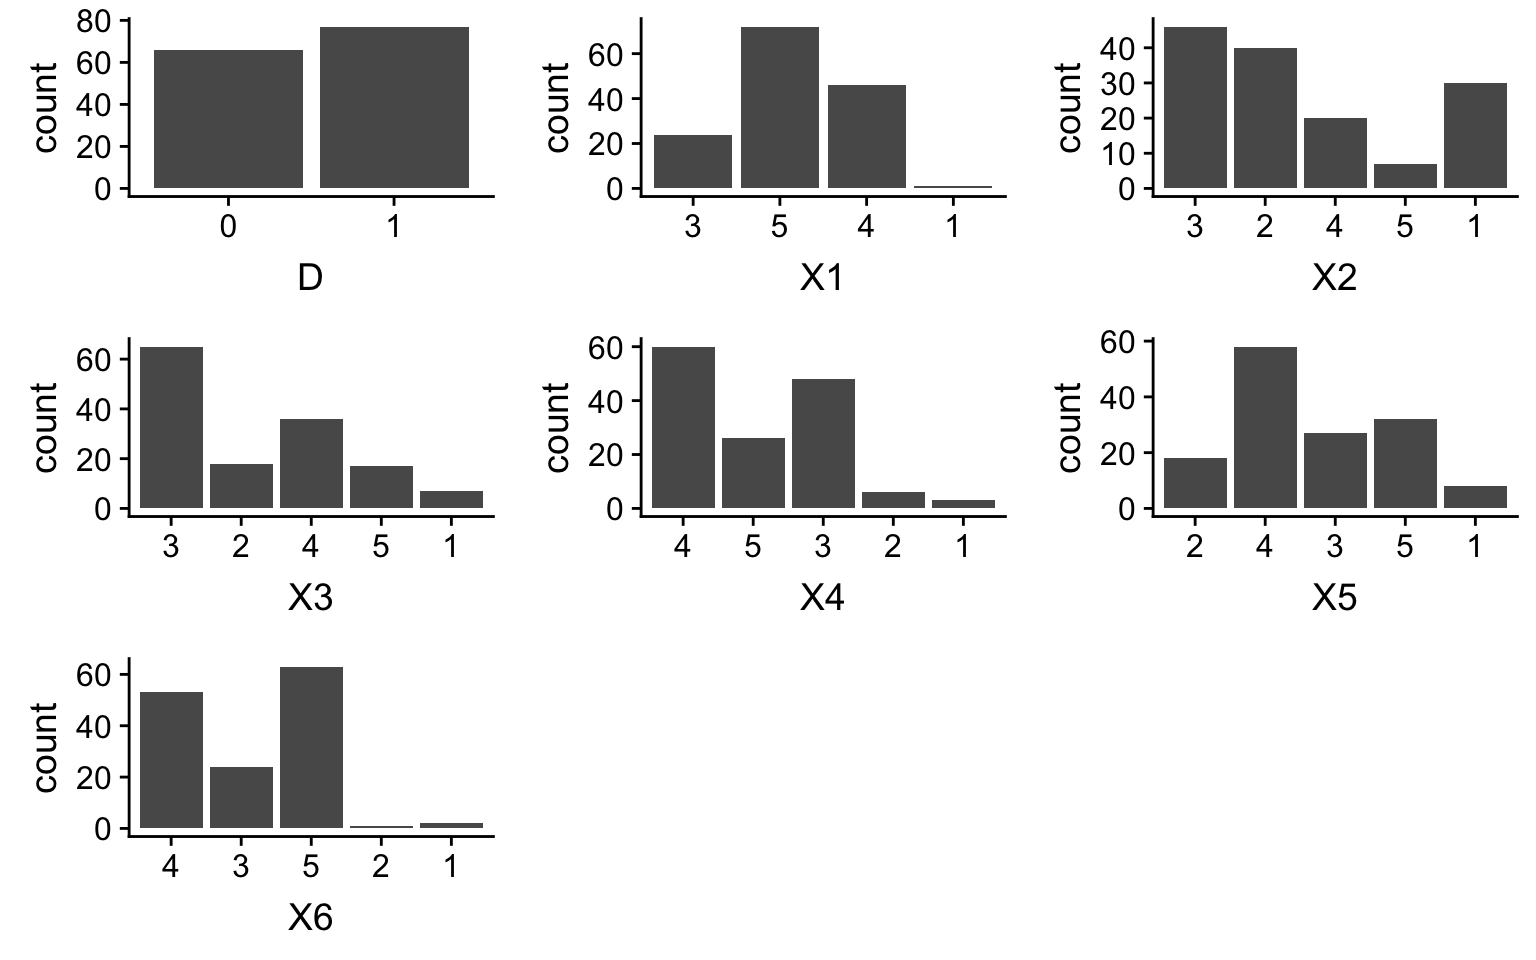
\includegraphics[width=1\linewidth]{Datasets_files/figure-latex/unnamed-chunk-8-1}

\hypertarget{mixed-categorical-and-numerical-attributes-1}{%
\subsection{Mixed: categorical and numerical
attributes}\label{mixed-categorical-and-numerical-attributes-1}}

\hypertarget{less-than-10-attributes-4}{%
\subsubsection{Less than 10
attributes}\label{less-than-10-attributes-4}}

\hypertarget{abalone}{%
\paragraph{Abalone}\label{abalone}}

Predicting the age of abalone from physical measurements. The age of
abalone is determined by cutting the shell through the cone, staining
it, and counting the number of rings through a microscope -- a boring
and time-consuming task. Other measurements, which are easier to obtain,
are used to predict the age. Further information, such as weather
patterns and location (hence food availability) may be required to solve
the problem.

From the original data examples with missing values were removed (the
majority having the predicted value missing), and the ranges of the
continuous values have been scaled for use with an ANN (by dividing by
200).

\begin{itemize}
\tightlist
\item
  \textbf{Source}:
  \href{http://archive.ics.uci.edu/ml/datasets/Abalone}{UCI Machile
  Learning Repository}
\item
  \textbf{Number of rows}: 4177
\item
  \textbf{Number of attributes}: 8
\end{itemize}

\textbf{Description of the attributes:}

\begin{verbatim}
## `stat_bin()` using `bins = 30`. Pick better value with `binwidth`.
## `stat_bin()` using `bins = 30`. Pick better value with `binwidth`.
## `stat_bin()` using `bins = 30`. Pick better value with `binwidth`.
## `stat_bin()` using `bins = 30`. Pick better value with `binwidth`.
## `stat_bin()` using `bins = 30`. Pick better value with `binwidth`.
## `stat_bin()` using `bins = 30`. Pick better value with `binwidth`.
## `stat_bin()` using `bins = 30`. Pick better value with `binwidth`.
\end{verbatim}

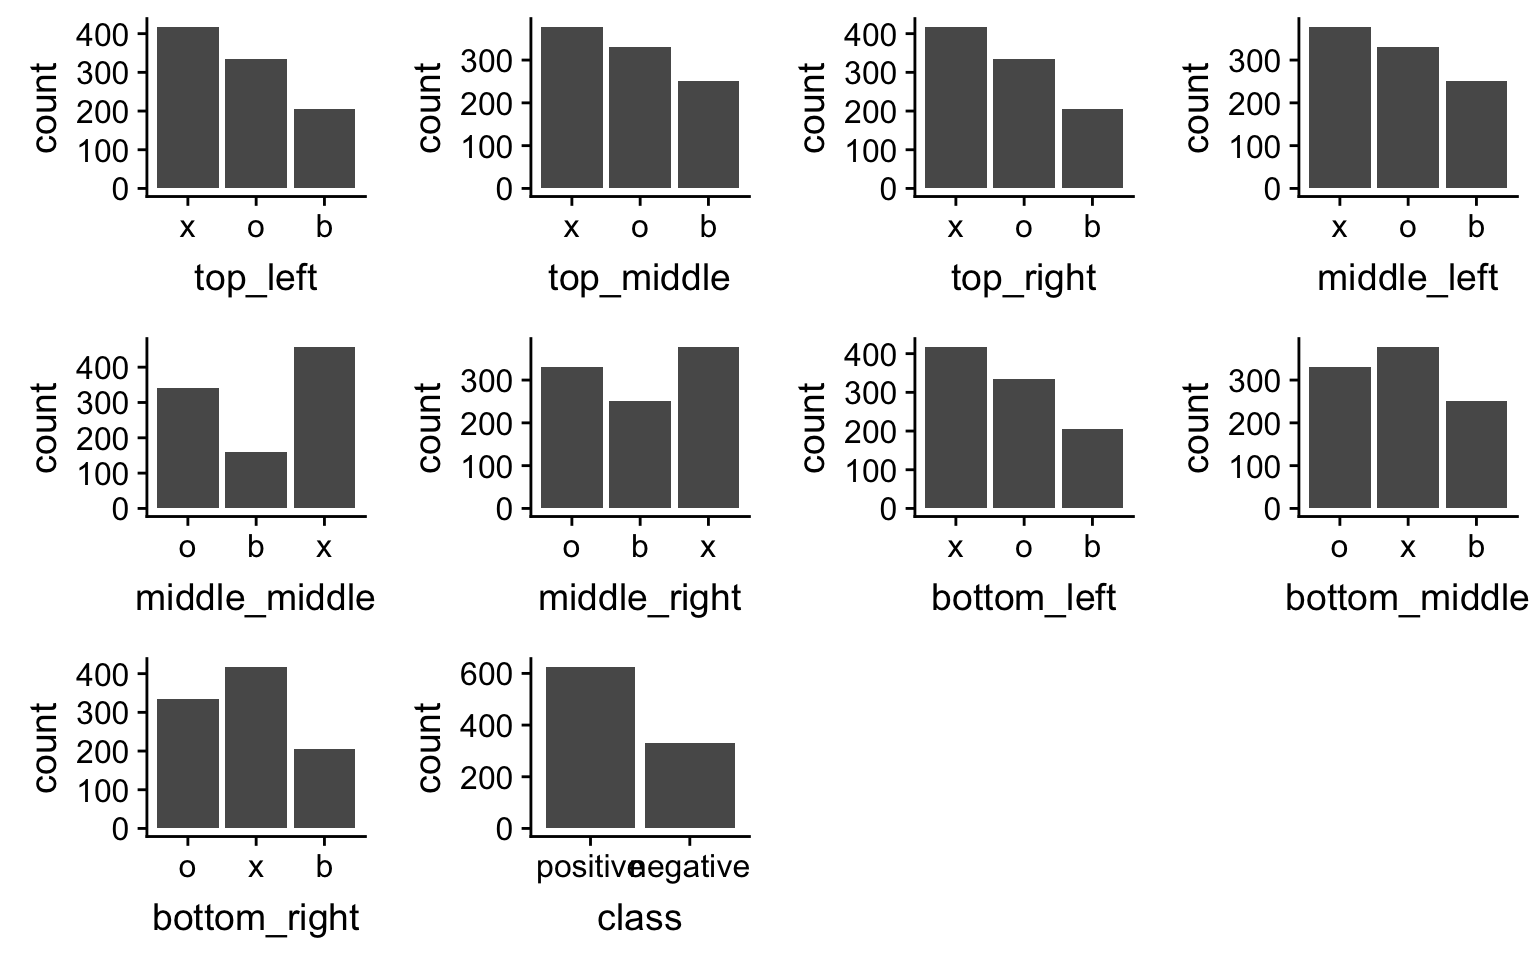
\includegraphics[width=1\linewidth]{Datasets_files/figure-latex/unnamed-chunk-9-1}

\hypertarget{life-expectancy}{%
\paragraph{Life expectancy}\label{life-expectancy}}

\begin{Shaded}
\begin{Highlighting}[]
\KeywordTok{ggplot}\NormalTok{(life_expectancy, }\KeywordTok{aes}\NormalTok{(male, female)) }\OperatorTok{+}\StringTok{ }
\StringTok{  }\KeywordTok{geom_point}\NormalTok{(}\KeywordTok{aes}\NormalTok{(}\DataTypeTok{color =}\NormalTok{ continent)) }
\end{Highlighting}
\end{Shaded}

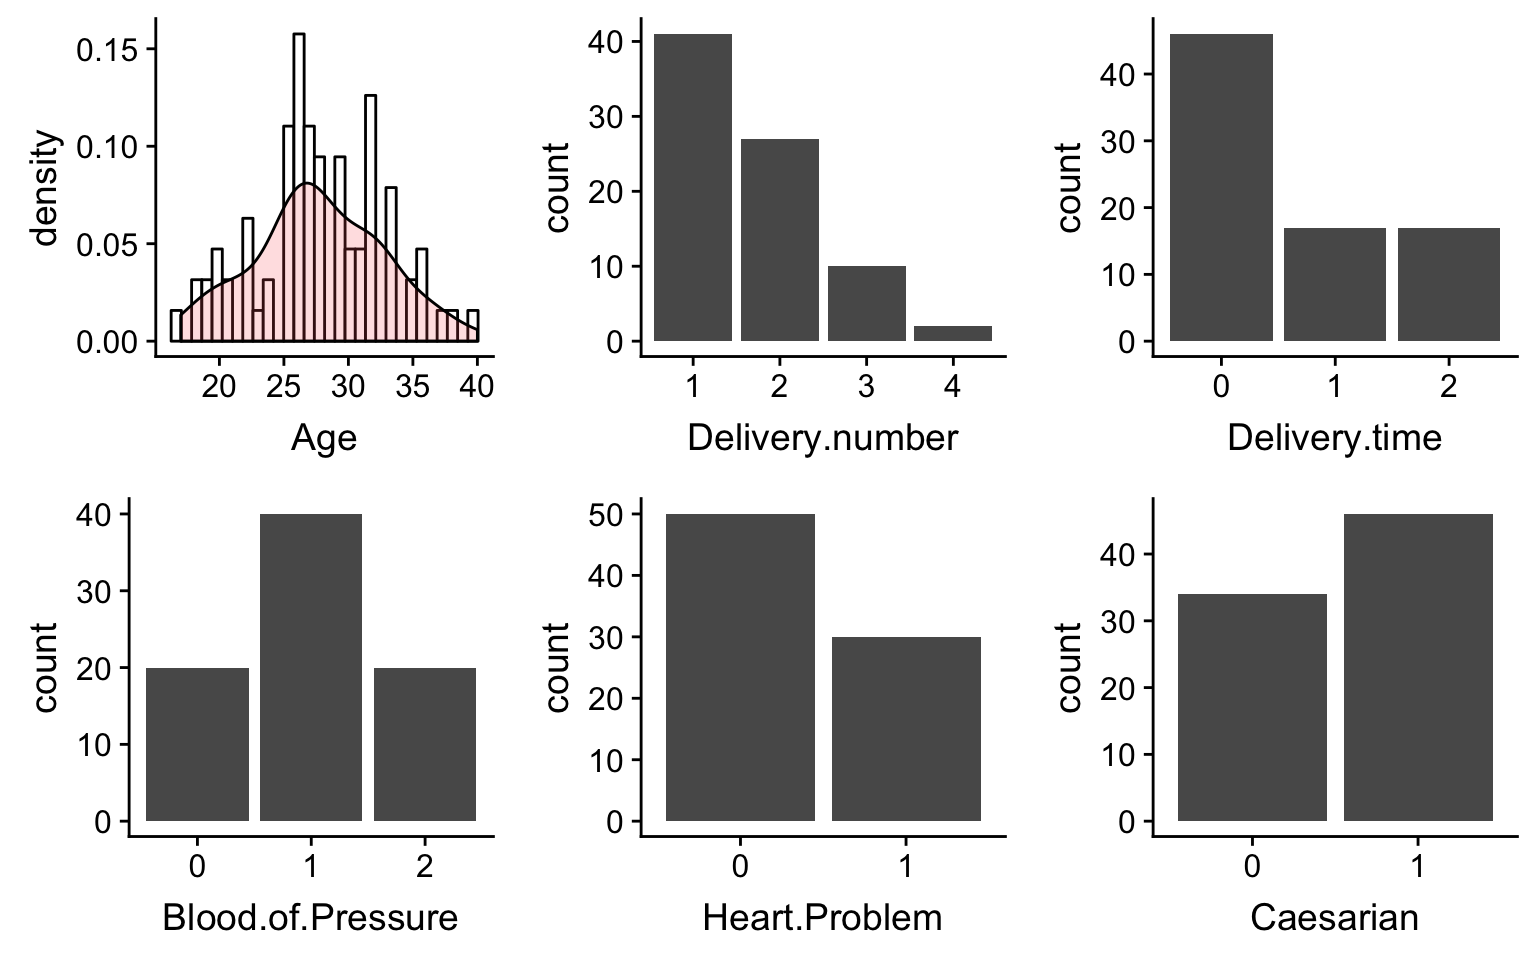
\includegraphics[width=1\linewidth]{Datasets_files/figure-latex/unnamed-chunk-10-1}

\hypertarget{or-more-attributes-4}{%
\subsubsection{10 or more attributes}\label{or-more-attributes-4}}

\hypertarget{numeric-attributes-1}{%
\subsection{Numeric attributes}\label{numeric-attributes-1}}

\hypertarget{less-than-10-attributes-5}{%
\subsubsection{Less than 10
attributes}\label{less-than-10-attributes-5}}

\hypertarget{life-expectancy-1}{%
\paragraph{Life expectancy}\label{life-expectancy-1}}

\begin{Shaded}
\begin{Highlighting}[]
\KeywordTok{ggplot}\NormalTok{(life_expectancy, }\KeywordTok{aes}\NormalTok{(male, female)) }\OperatorTok{+}\StringTok{ }
\StringTok{  }\KeywordTok{geom_point}\NormalTok{(}\KeywordTok{aes}\NormalTok{(}\DataTypeTok{color =}\NormalTok{ continent)) }
\end{Highlighting}
\end{Shaded}

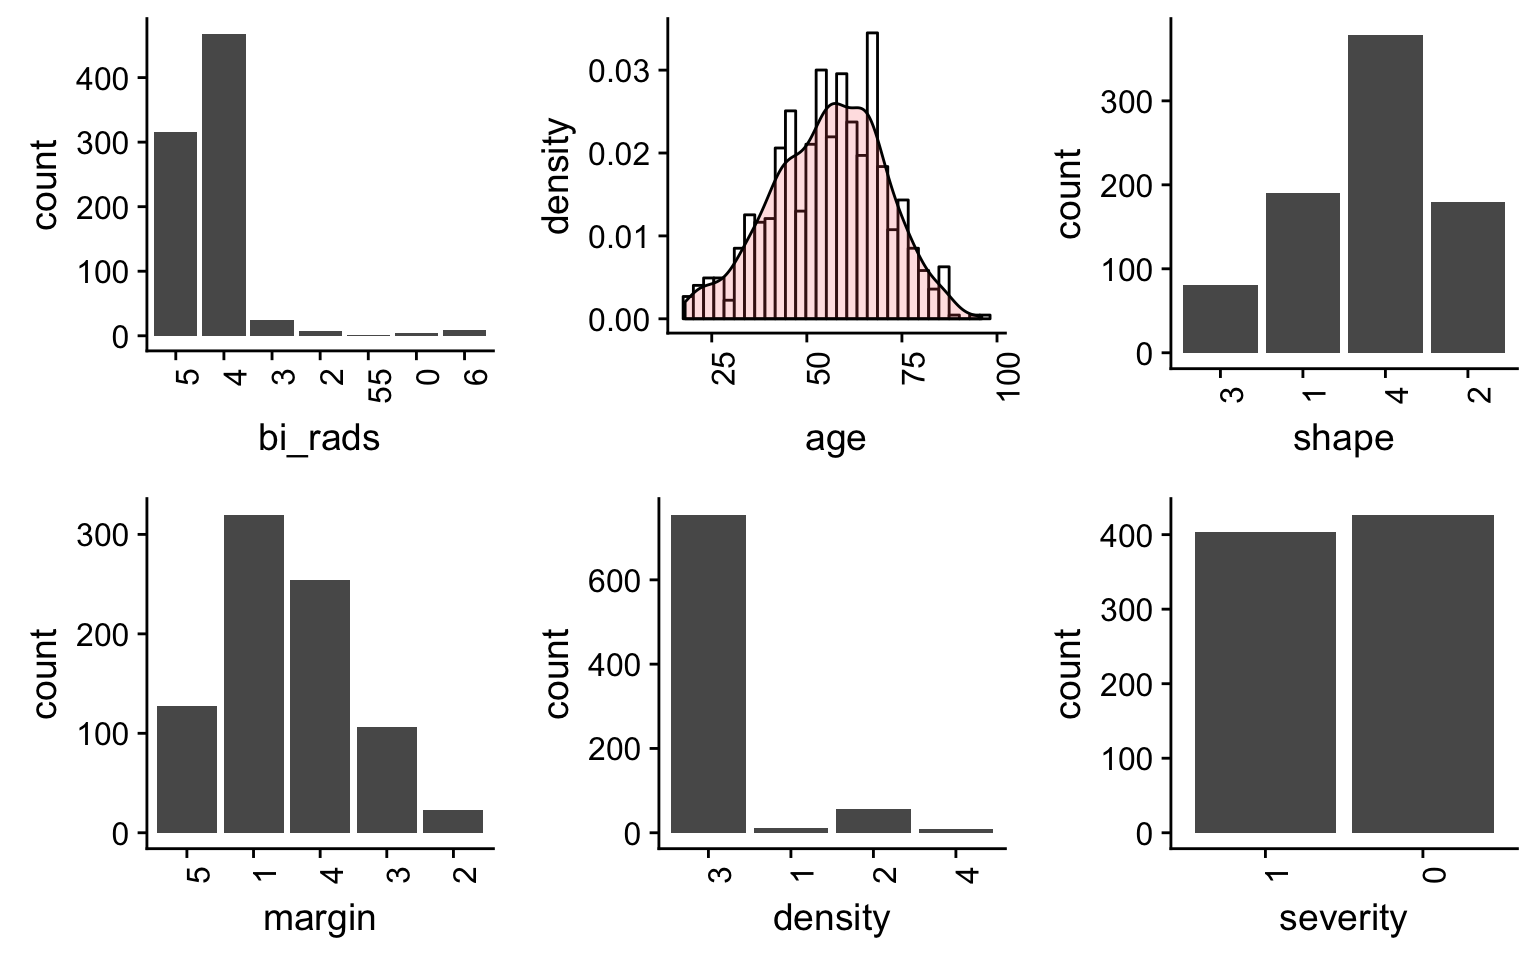
\includegraphics[width=1\linewidth]{Datasets_files/figure-latex/unnamed-chunk-11-1}

\hypertarget{or-more-attributes-5}{%
\subsubsection{10 or more attributes}\label{or-more-attributes-5}}

This database encodes the complete set of possible board configurations
at the end of tic-tac-toe games, where ``x'' is assumed to have played
first. The target concept is ``win for x'' (i.e., true when ``x'' has
one of 8 possible ways to create a ``three-in-a-row'').

\begin{itemize}
\tightlist
\item
  \textbf{Source}:
  \href{http://archive.ics.uci.edu/ml/datasets/Tic-Tac-Toe+Endgame}{UCI
  Machile Learning Repository}
\item
  \textbf{Number of rows}: 958
\item
  \textbf{Number of attributes}: 9
\end{itemize}

\textbf{Description of the attributes:}

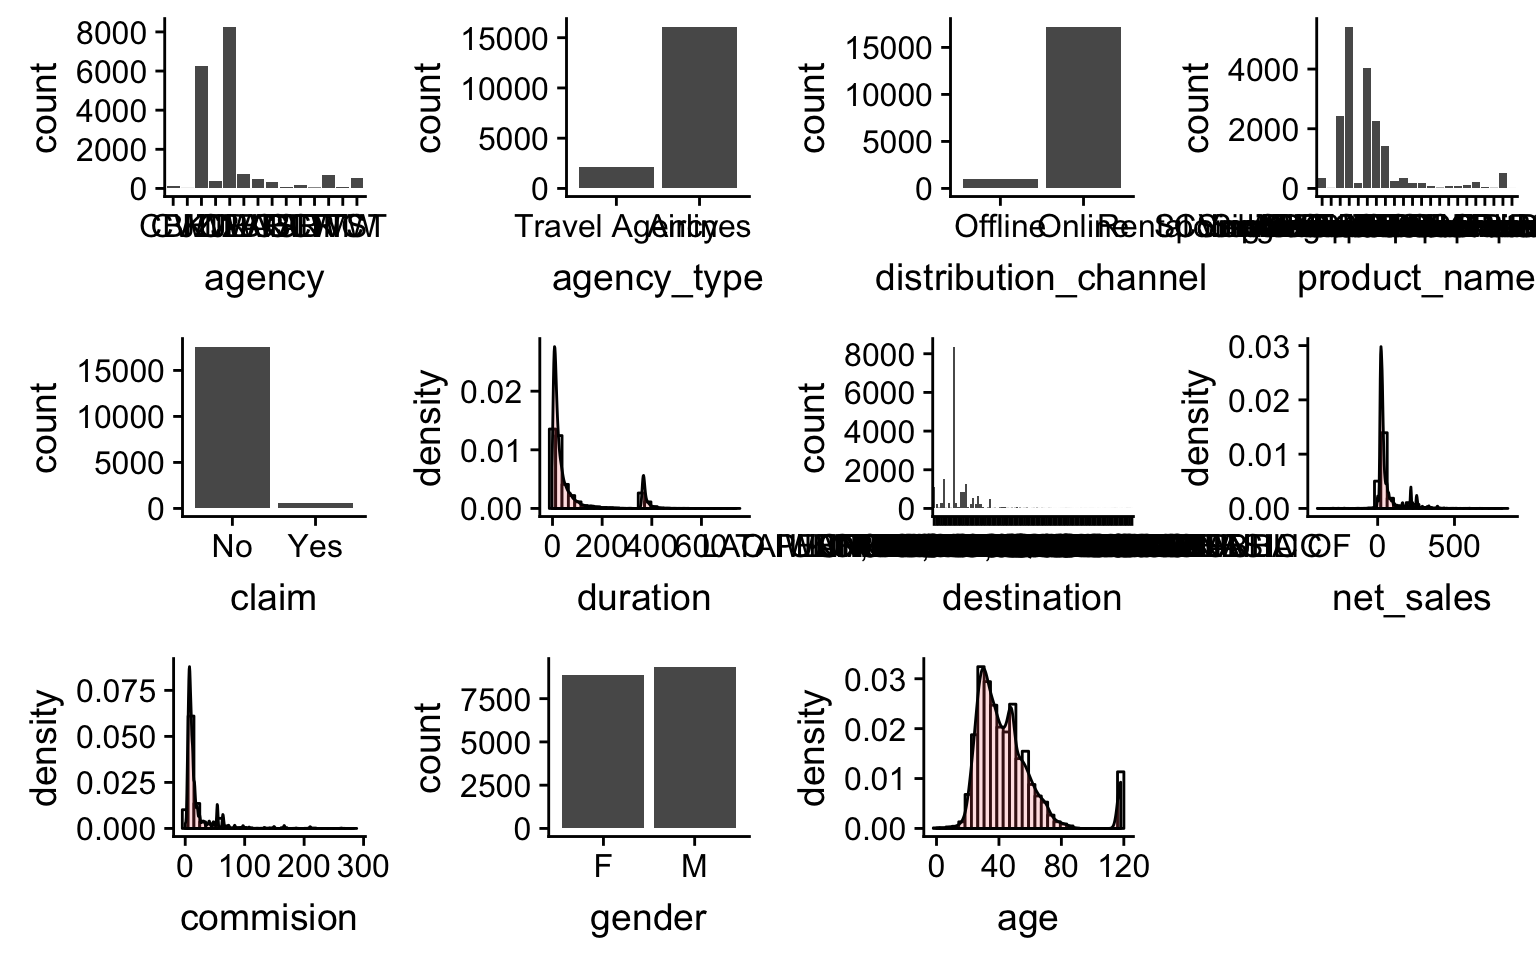
\includegraphics[width=1\linewidth]{Datasets_files/figure-latex/unnamed-chunk-12-1}

\hypertarget{notes}{%
\section{Notes}\label{notes}}

Changes to the original datasets if any:


\end{document}
